% Author: Dr. Matthias Jung, DL9MJ
% Year: 2020
\documentclass[convert = false, border=5pt]{standalone}
\usepackage{fontspec}
\setmainfont{Roboto}
\usepackage[siunitx, straightvoltages, europeanresistors, european inductor]{circuitikzgit}
\usepackage{tikz}


\usepackage{tikz,pgfplots}
\usepgfplotslibrary{fillbetween}

\begin{document} 
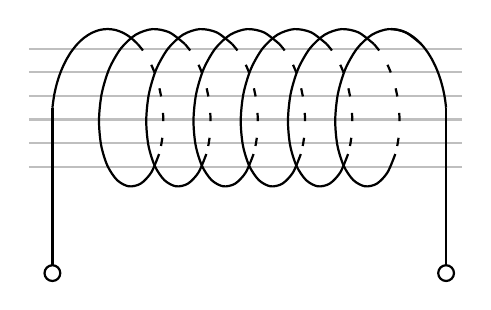
\begin{tikzpicture}

    \begin{scope}[gray!50, thick]
        \draw (-1,0.75) -- (4.5,0.75);
        %\draw (-1,1.25) -- (4.5,1.25);
        %\draw (4.5,0.75) arc (-90:90:0.25) ;
        %\draw (-1,1.25) arc (90:270:0.25) ;
        %
        \draw (-1,0.45) -- (4.5,0.45);
        %\draw (-1,1.55) -- (4.5,1.55);
        %\draw (4.5,0.45) arc (-90:90:0.55) ;
        %\draw (-1,1.55) arc (90:270:0.55) ;
        %
        \draw (-1,0.15) -- (4.5,0.15);
        %\draw (-1,1.85) -- (4.5,1.85);
        %\draw (4.5,0.15) arc (-90:90:0.85) ;
        %\draw (-1,1.85) arc (90:270:0.85) ;
        %
        \draw (-1,-0.75) -- (4.5,-0.75);
        %\draw (-1,-1.25) -- (4.5,-1.25);
        %\draw (4.5,-1.25) arc (-90:90:0.25) ;
        %\draw (-1,-0.75) arc (90:270:0.25) ;
        %
        \draw (-1,-0.45) -- (4.5,-0.45);
        %\draw (-1,-1.55) -- (4.5,-1.55);
        %\draw (4.5,-1.55) arc (-90:90:0.55) ;
        %\draw (-1,-0.45) arc (90:270:0.55) ;
        %
        \draw (-1,-0.15) -- (4.5,-0.15);
        %\draw (-1,-1.85) -- (4.5,-1.85);
        %\draw (4.5,-1.85) arc (-90:90:0.85) ;
        %\draw (-1,-0.15) arc (90:270:0.85) ;
        %
    \end{scope}
    
    % Define a formula for the coil.
    % This is what the numbers mean:
    % A ... how far the rings are apart
    % B ... how much from the side the rings are seen (try 0 and the same as the radius)
    % C ... radius of the rings
    \def\coil#1{
        % A                   B
        {0.3 * (2*#1 + \t) + 0.55*sin(\t * pi r))},
        % C
        {1.0 * cos(\t * pi r)}
    }

    % Draw the part of the coil behind the rectangle
    \foreach \n in {0,1,...,5} {
        \draw[domain={0.2:0.7},smooth,variable=\t,samples=15, loosely dashed, thick]
            plot (\coil{\n}); 
        }

    % Draw the part of the coil in front of the rectangle
    \foreach \n in {0,1,...,5} {
        \draw[domain={0.7:2.2},smooth,variable=\t,samples=15, thick]
            plot (\coil{\n});
        }

    \draw[domain={ 0.0:0.5},smooth,variable=\t,samples=15,thick] plot (\coil{6});
    \draw[domain={-0.5:0.2},smooth,variable=\t,samples=15,thick] plot (\coil{0});
    \draw[thick](-0.7,0) -- (-0.7,-2);
    \draw[thick](4.3,0) -- (4.3,-2);
    \draw[thick](4.3,-2.1) circle (0.1);
    \draw[thick](-0.7,-2.1) circle (0.1);


\end{tikzpicture}

\end{document}

